\subsection{LMFormer: Lane based Motion Prediction Transformer}
\label{ssec:lmformer}

LMFormer~\cite{lmformerYadav2025} is a fully query-centric, transformer-based architecture for joint multi-agent trajectory forecasting. It ingests both static lane segments and dynamic motion vectors in their local frames, embeds them via learnable Fourier features, and processes them through self- and cross-attention blocks before iteratively decoding multiple modes for each agent. The high-level architecture is shown in \autoref{fig:lmformer_arch}.

\begin{figure}[ht]
  \centering
  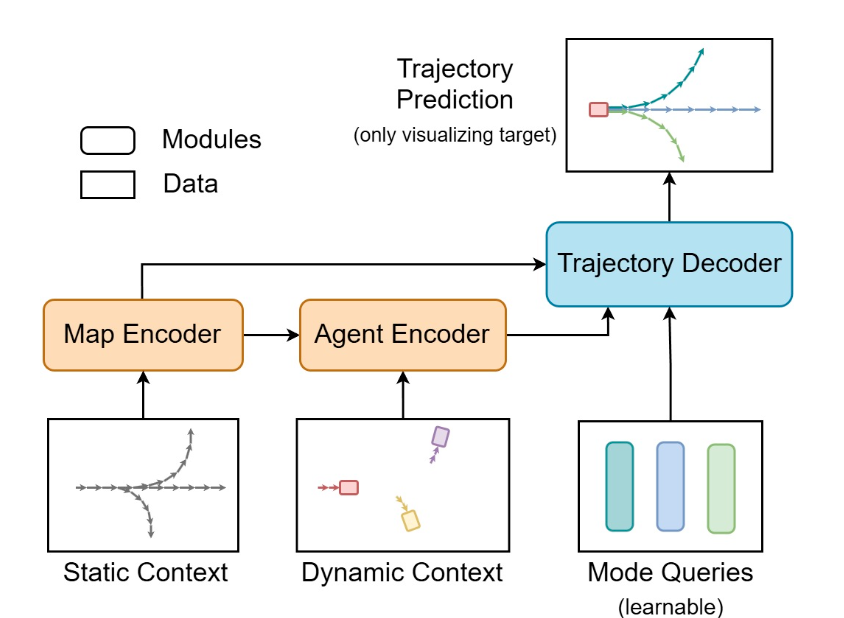
\includegraphics[width=0.8\textwidth]{figures/lmformer_arch.png}
  \caption{LMFormer architecture: transformer encoders for static and dynamic contexts \& recurrent cross-attention decoder with coarse-to-fine refinement~\cite{lmformerYadav2025}.}
  \label{fig:lmformer_arch}
\end{figure}


\subsubsection{Encoder}
The encoder leverages the asymmetric relationship between static and dynamic contexts: while static lane geometry is independent of dynamic agent states, agent behavior is heavily influenced by road structure. This motivates a two-stage design where static context is encoded first, then incorporated into dynamic agent processing. Following the original architecture~\cite{lmformerYadav2025}, all scalar inputs are embedded using learnable Fourier features before processing through specialized attention modules.
\begin{figure}[H]
  \centering
  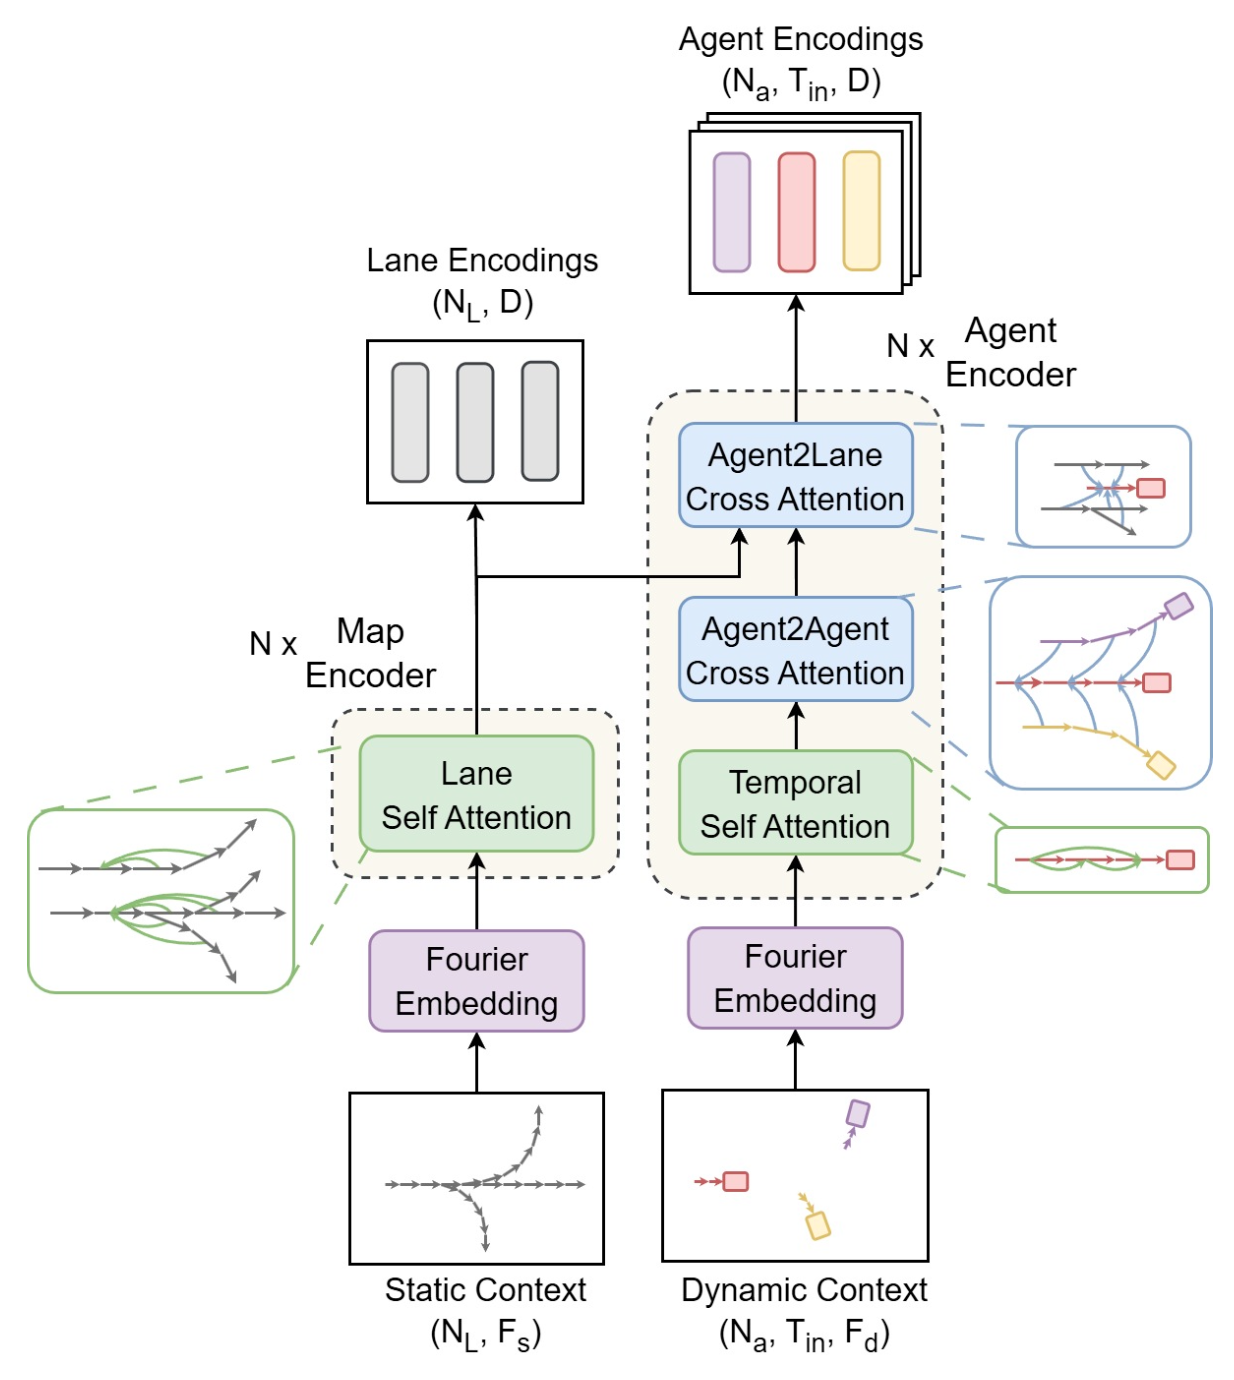
\includegraphics[width=0.6\textwidth]{figures/lmformer_arch_encorder.png}
  \caption{LMFormer encoder: learnable Fourier embeddings, lane self-attention, agent temporal and cross-attentions~\cite{lmformerYadav2025}.}
  \label{fig:lmformer_arch_encoder}
\end{figure}

\subsubsubsection{Learnable Fourier Embeddings}
All scalar inputs—lane-segment lengths, relative headings, time offsets, motion-vector norms, and relative descriptors—are lifted with \emph{learnable Fourier features}~\cite{li2021llearnableFourier}:
\begin{equation}
  \label{eq:learnable_fourier_embedding}
\mathbf{x} \mapsto \text{GeLU}\left(\mathbf{W}_A \begin{bmatrix} \sin(2\pi \mathbf{x} \mathbf{W}_f^T) \oplus \cos(2\pi \mathbf{x} \mathbf{W}_f^T) \end{bmatrix} + \mathbf{B}_\varphi\right) + \mathbf{B}_\psi
\end{equation}
where all \(\mathbf{W}_\bullet\) and \(\mathbf{B}_\bullet\) are learnable parameters:
\begin{itemize}[leftmargin=*]
    \item \(\mathbf{W}_f\) encodes which harmonic frequencies are emphasized for each scalar input dimension,
    \item \(\mathbf{W}_A\) represents the amplitude of each frequency in the harmonic basis,
    \item \(\mathbf{B}_\varphi\) are learnable phase shifts for each harmonic, and \(\mathbf{B}_\psi \) is a learnable bias of the final embedding.
\end{itemize}
This harmonic basis lets later attention layers pick up patterns at various task-adaptive spatio-temporal frequencies. Unlike fixed sinusoidal embeddings, the learnable frequencies in \(\mathbf{W}_f\) adapt during training to capture the most informative scales for trajectory prediction—from fine-grained local maneuvers to coarse lane-following behaviors.


\begin{itemize}[leftmargin=*]
    \item \textbf{Map (Lane) Encoder:}
        Applies \(N_{es}\) layers of multi-headed self-attention over \(N_L = K \cdot L\) lane-segment tokens to capture  topological and geometric relations between lane segments. Each segment is represented by its query-centric Fourier embeddings, with relative position embeddings incorporated into the keys/values to maintain spatial relationships. The resulting \emph{static scene encodings} are \(\mathbf{E}_s \in \mathbb{R}^{N_L \times D}\).
  \item \textbf{Agent Encoder:}
        Stacks three attention modules over \(N\) agent tokens with \(T_{p}\) timesteps:
        \begin{enumerate}
          \item Temporal self-attention models the temporal dependencies of each agent, allowing each agent to attend to its own past motion history.
          \item Agent-agent cross-attention to model social interactions between agents per timestep, enabling agents to attend to the encodings of other agents at the same timestep.
          \item Agent-lane cross-attention to the \(N_L \times D \) dimensional lane encodings (keys + values) and dynamic agent encodings (queries).
        \end{enumerate}
        The encoder repeats this triad \(N_{ed}\) times, producing \emph{agent encodings} \(\mathbf{E}_d \in \mathbb{R}^{N \times T_{p} \times D}\).
\end{itemize}

\subsubsection{Recurrent Cross-Attention Decoder}

To facilitate multimodal trajectory prediction, LMFormer introduces learnable mode queries where each query corresponds to a distinct trajectory for every agent. The decoder employs a two-level strategy combining iterative refinement across \(N_{\text{dec}}\) stacked layers with autoregressive generation within each layer. Inspired by DAB-DETR's coarse-to-fine anchor refinement~\cite{liu2022dabdetr}, early layers establish coarse trajectory patterns while later layers add fine-grained details, maintaining temporal coherence and social consistency.

\begin{figure}[ht]
  \centering
  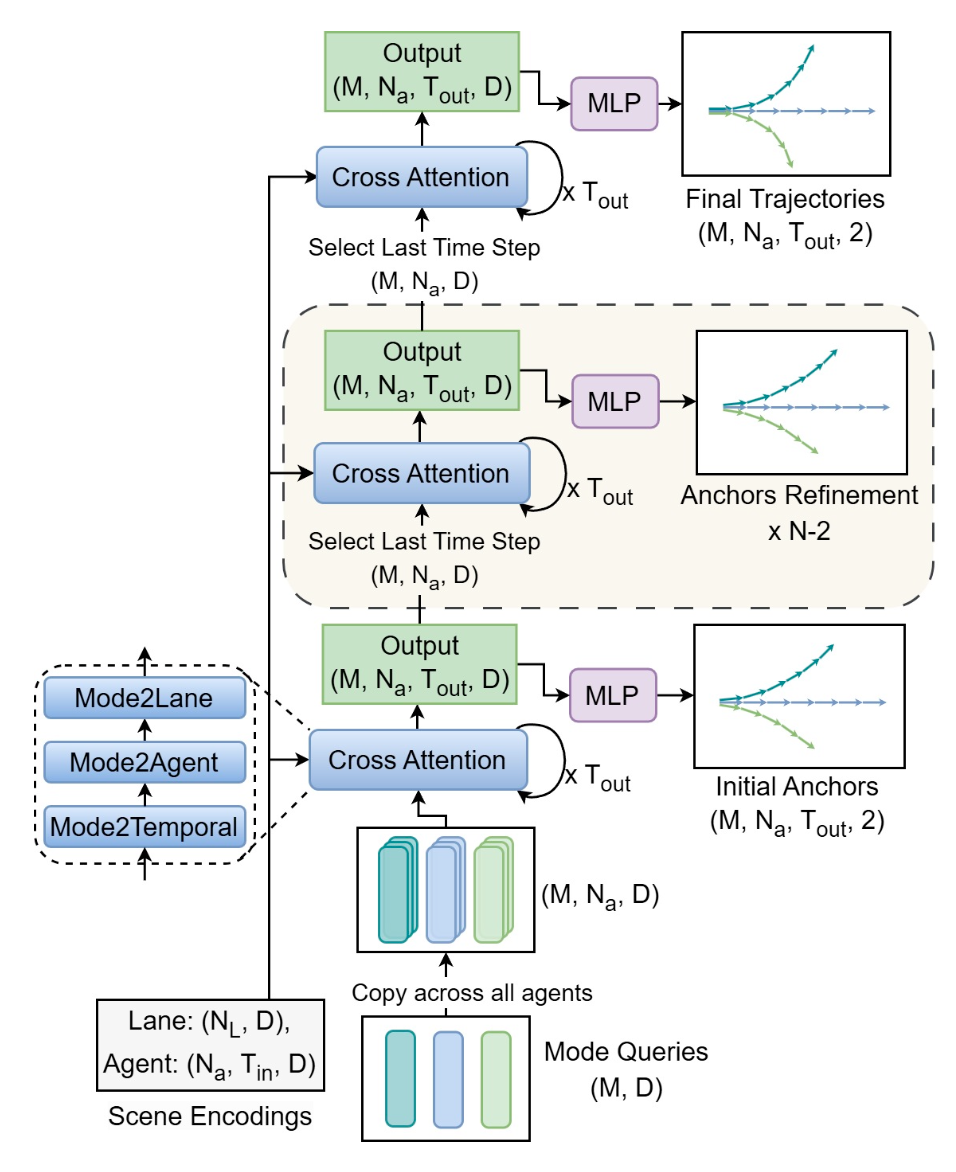
\includegraphics[width=0.6\textwidth]{figures/lmformer_arch_decoder.png}
  \caption{\cite{lmformerYadav2025}~LMFormer decoder: recurrent mode-query cross-attention modules that iteratively generate future motion vectors.}
  \label{fig:lmformer_arch_decoder}
\end{figure}

The architecture incorporates recurrent temporal decoding (\(\times T_f\)) within cross-attention modules, where each recurrent loop updates both query position and content, similar to CASPFormer~\cite{caspformerYadav2024}. Only the final timestep representations from each block are propagated forward, creating a bottleneck that forces the model to compress learned temporal dynamics into a compact representation. Each motif employs three cross-attention modules to capture various interactions:
\begin{itemize}[leftmargin=*]
  \item \textbf{Mode2Temporal Cross-Attention:} Aggregates temporal information of agent encodings (keys/values) along the time-axis to mode queries, aligning each behavioral hypothesis with the agent's observed motion history.

  \item \textbf{Mode2Agent Cross-Attention:} Models social interactions where each mode of an agent attends to the same mode of other agents at the same historic timestep, ensuring multi-modal futures are grounded in historic social context.

  \item \textbf{Mode2Lane Cross-Attention:} Grounds trajectory modes in static road geometry by letting mode queries attend to lane segment encodings, incorporating drivable directions, topology constraints, and map alignment.
\end{itemize}

Each decoder block \(i \in \{1, \ldots, N_{\text{dec}}\}\) maintains a query tensor \(\mathbf{Q}^{(i)} \in \mathbb{R}^{M \times N \times T_f \times D}\) where \(M\) is the number of modes per agent.

\textbf{Output Formulation.} Following \cite{lmformerYadav2025}, every mode query ultimately predicts a \emph{motion-vector chain}
\begin{equation}
\mathcal{T}_{out}^{a,m} = \bigl[(V_1^{a,m},S_1^{a,m}),\dots,(V_{T_f}^{a,m},S_{T_f}^{a,m})\bigr],
\end{equation}
where \(V_t^{a,m}=[P_{t-1}^{a,m},P_t^{a,m}]\) is a displacement vector and \(S_t^{a,m}\in\mathbb{R}^{2}\) its uncertainty. Each \( (V_t,S_t) \) pair parameterises one component of a \emph{Laplacian mixture} density. To elucidate the workings within the decoder, we present its simplified algorithmic description in \autoref{alg:lmformer_decoder}.

% TODO:integrate the algorithm into the textual and conceptual description
\begin{algorithm}[H]
\caption{LMFormer Recurrent Cross-Attention Decoder}
\label{alg:lmformer_decoder}
\begin{algorithmic}[1]
\REQUIRE Agent encodings \(\mathbf{E}_d \in \mathbb{R}^{N \times T_{p} \times D}\), Lane encodings \(\mathbf{E}_s \in \mathbb{R}^{N_L \times D}\), Learned Mode anchors \(\mathbf{A} \in \mathbb{R}^{M \times D}\)
\ENSURE Trajectory sets \(\{\mathcal{T}_{out}^{(i)}\}_{i=1}^{N_{\text{dec}}}\)
\STATE \(\mathbf{q} \leftarrow \text{repeat}(\mathbf{A}, N)\) \(\triangleright\) Initialize mode queries \((M, N, D)\)
\FOR{\(i = 1\) \textbf{to} \(N_{\text{dec}}\)}
    \STATE \(\mathbf{Q}_{\text{seq}}^{(i)} \leftarrow \text{zeros}(M, N, T_f, D)\)
    \FOR{\(t = 1\) \textbf{to} \(T_f\)}
        \STATE \(\triangleright\) \textbf{Mode2Temporal}
        \STATE \(\mathbf{q}\leftarrow \text{CrossAttn}(\mathbf{q}, K=V=\mathbf{E}_d[\text{same } n, \tau = 1\dots, T_p, :])\)
        \STATE \(\triangleright\) \textbf{Mode2Agent}
        \STATE \(\mathbf{q}\leftarrow \text{CrossAttn}(\mathbf{q}, K=V=\mathbf{E}_d[\tilde{n}=1\dots n, \text{same } \tau, :])\)
        \STATE \(\triangleright\) \textbf{Mode2Lane}
        \STATE \(\mathbf{q}\leftarrow \text{CrossAttn}(\mathbf{q}, K=V=\mathbf{E}_s)\)
        \STATE \(\mathbf{Q}_{\text{seq}}^{(i)}[:, :, t, :] \leftarrow \mathbf{q}\)
    \ENDFOR
    \STATE \(\mathcal{T}_{out}^{(i)} \leftarrow \text{MLP}(\mathbf{Q}_{\text{seq}}^{(i)})\) \(\triangleright\) \((M, N, T_f, 4)\)
\ENDFOR
\end{algorithmic}
\end{algorithm}

\subsubsubsection{Loss formulation}
LMFormer re-uses winner-takes-all regression loss from~\autoref{eq:caspformer_regression_loss}, combined with the cross-entropy loss to update mode probabilities from~\autoref{eq:caspformer_classification_loss} but supervises \emph{every} refinement layer (except the first) to encourage iterative coarse-to-fine anchor refinement:
\begin{equation}
  \mathcal{L}
  = \lambda\,\mathcal{L}_{cls}
    + \sum_{n=2}^{N_{\text{dec}}}\mathcal{L}_{reg}^{(n)},
  \label{eq:lm_loss}
\end{equation}
where \(\lambda\) balances classification against regression~\cite{lmformerYadav2025}.

% allowed to edit below:
\subsubsection{Discussion} % Here our critique and qualitative analysis of LMFormer.

\begin{description}[itemsep=0.5em]

\item[\textbf{Static Context Limitations}]
  \item Contrary to the claim in~\cite{lmformerYadav2025} that connections between segments with similar heading should dominate, the learnable Fourier encoding should be capable of representing much more complex relations between segments. As Eq.~\eqref{eq:learnable_fourier_embedding} suggests, the learnable Fourier+MLP can capture relations beyond mere heading similarity. The authors used this hypothesis to justify not reaching SOTA performance on minFDE@1 on nuScenes, claiming that the model might fail to forecast trajectories not aligned with lane segments.\\

Lane graphs are intrinsically sparse, replacing dense attention with deformable or other sparse attention schemas would reduce this block's cost from \(\mathcal{O}(N_L^2)\) to \(\mathcal{O}(N_L K_s)\) without harming accuracy, mirroring the gains CASPFormer achieved in the raster domain.\\
  Their ablation studies showed that long-range dependencies in lane encodings do not appear significant, which supports our claim, that encoding mechanisms that focus on local relationships and sparsely on long-range relationships might be beneficial. \cite{qcnetZhou2023} employed graph neural networks to model the lane graph, which would be a potential alternative to the self-attention mechanism employed in LMFormer's map encoder.
  We question why the authors only encoded lane segments while other static scene elements listed in \autoref{tab:polyline-types} were not included in the static scene encoder, as they obviously carry important information for trajectory forecasting. However, we acknowledge that lanes play a dominant role in conditioning feasible trajectories during decoding, so it might be worthwhile to decode the static scene context in a way that allows the resulting latents to be decomposed into lane segments and other static scene elements.\\

As~\cite{lmformerYadav2025} notes, future work could explore encoding explicit physical feasibility constraints (e.g., speed limits) inside the decoder.

\item[\textbf{Offset-based Refinement}]
LMFormer predicts a \emph{full}, absolute trajectory at every decoder stage. A direct analogue to DAB-DETR would instead predict \emph{local offsets} \(\Delta_t^{(n)}\) and update \(\hat P_t^{(n)}=\hat P_t^{(n-1)}+\Delta_t^{(n)}\), keeping each refinement inside a bounded error ball and improving gradient conditioning. Employing a residual formulation is generally seen as a measure to improve gradient stability, allow for faster convergence and smoother paths~\cite{liu2022dabdetr}. While~\cite{lmformerYadav2025} notes that the autoregressive nature necessary for motion forecasting conflicts with the offset-based approach, we cannot understand why this would be the case.

% TODO: this does not belong to this item


\item[\textbf{Velocity-Position Decoupling and Optimization}]
As~\cite{lmformerYadav2025} notes, it would be beneficial to redict velocity mixtures in a separate head. Velocities are usually provided as ground-truth and could hence be optimized directly, furthermore integrating them would yield a second branch to predict trajectory positions, grounding these predictions in the velocity profile and contributing to physical continuity.

While~\cite{lmformerYadav2025} weighs the regression losses across all refinement layers uniformly, we believe that later layers should dominate the regression loss. This is because early layers primarily establish coarse trajectory patterns, while later layers refine these patterns into fine-grained, multi-modal trajectories. Furthermore, the gradient emitted from the loss of the later layers will also affect all previous layers.

\item[\textbf{Geometric Symmetries \& Multi-Agent Capabilities}]
The architecture preserves all symmetries as introduced in \autoref{sssec:qc_geometric_perspective}. These properties allow the same cached scene encoding to serve \emph{all} agents and \emph{all} successive frames, a capability absent in all agent-centric architectures.



\item[\textbf{Generalization \& Data Diversity}]
The authors remarked on limited generalization capabilities when cross-testing on other datasets. This is exacerbated by the lack of diverse training data and unbalanced data distributions in nuScenes, where some maneuvers occur less frequently. UniTraj already provides a classification of maneuver types (which could be extended) such that those that are underrepresented could be oversampled during training to improve generalization capabilities. This supports our remarks in \autoref{sec:data_methodology} on why a unified dataset via a framework like UniTraj will be necessary to achieve improved generalization capabilities.

The authors furthermore noted the need for targeted data augmentation strategies to improve robustness and mode diversity; such augmentation strategies would be a natural extension of the UniTraj framework, as these augmentations could benefit all sorts of trajectory forecasting models, not just LMFormer.

\end{description}

\subsubsubsection{Pros}
\begin{itemize}[leftmargin=*, label=\greenoplus]
  \item Fully query-centric, preserving \(\mathrm{SE}(2)\!\rtimes\!\mathbb{R}\) invariance end-to-end.
  \item Joint multi-agent decoding with shared static context.
  \item Recurrent refinement yields temporally coherent, multi-modal trajectories.
  \item Managed to drastically reduce VRAM requirements compared to \cite{qcnetZhou2023}, as they trained on a single A100 GPU with 40GB VRAM, while QCNet required approx. 160GB VRAM for training.
\end{itemize}

\subsubsubsection{Cons}
\begin{itemize}[leftmargin=*, label=\redominus]
  \item Higher VRAM demand compared to CASPFormer due to larger key-value cache.
  \item Limited static context representation (lane-only tokens).
  \item Uniform loss weighting across refinement layers rather than emphasizing later stages.
  \item Generalization challenges across different datasets due to training data limitations.
  \item Employed only a single type of augmentation (flipping inputs along the driving direction).
\end{itemize}

\subsubsubsection{Relation to CASPNet \& CASPFormer}
CASPNet operates on raster grids and predicts per-pixel occupancies; CASPFormer adds deformable attention and vector outputs but retains an \emph{agent-centric} frame. LMFormer discards the raster backbone entirely, embraces the query-centric paradigm, and gains strict symmetry compliance and parallel multi-agent decoding—at the cost of a larger key-value cache and higher VRAM demand (\(\approx\)2x CASPFormer on nuScenes).

\newpage

